\section{Introduction}

\subsection{Overview}

Retrieval-Augmented Generation (RAG) has emerged as the dominant method to ground Large Language Model (LLM) generation outputs 
with retrieved external evidence in text-only settings \cite{tonmoy2024comprehensivesurveyhallucinationmitigation}.
Multimodal LLMs (MLLMs) capable of processing both text and visual content are becoming widely used,
yet existing and widely used RAG pipelines designed for text-only models cannot directly accomodate multimodal information as retrieved evidence for grounding generation.

\begin{figure}[H]
    \centering
    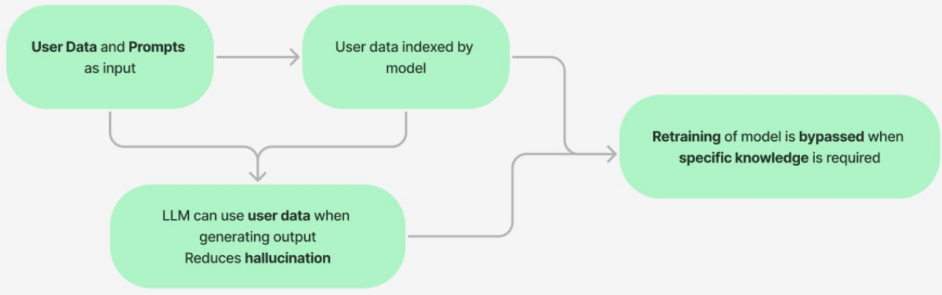
\includegraphics[width=0.95\textwidth]{images/1-intro/rag-rationale.png}
    \caption{Rationale behind RAG}
\end{figure}

\begin{figure}[H]
    \centering
    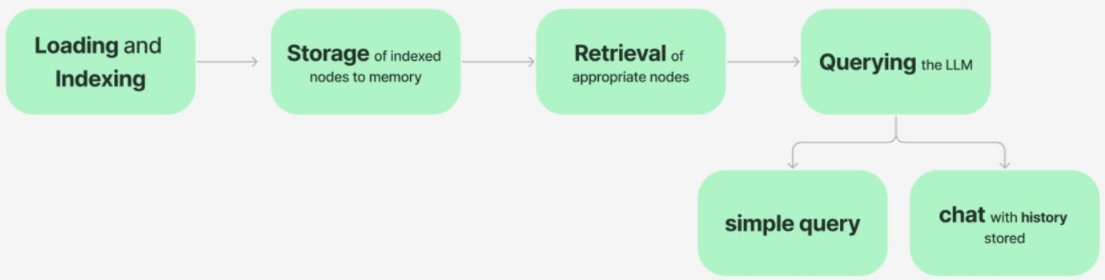
\includegraphics[width=0.85\textwidth]{images/1-intro/rag-text-pipeline.png}
    \caption{A typical text-based RAG pipeline}
\end{figure}

Consider a domain expert querying a MLLM on the fine-grained difference between two rare bird species,
an engineer asking a MLLM about specific designs on design plans in scanned blueprint documents,
or a doctor inspecting a patient's X-ray scans for structures that may appear in certain diseases with the help of a MLLM.
In these cases, relevant evidence in visual form cannot be retrieved for use with a MLLM when widely adopted text-only RAG pipelines are used.
Existing multimodal RAG pipelines demonstrate bias towards text instead of visual information and rely on captions that do not contain visual features,
or may not be able to capture fine-grained visual features precisely \cite{abootorabi-etal-2025-ask,lin2025mmembeduniversalmultimodalretrieval}.
This modality gap fundamentally limits the capabilties of RAG systems, and the application of RAG in domains where visual elements dominate,
as well as high-stakes domains where precision and accuracy are crucial.

Recent surveys have reviewed and documented the development of multimodal RAG and 
have noted advancements in graph storage structures and agentic frameworks \cite{gao2026scalingcontextsurveymultimodal}.
However, limitations in existing approaches may bring limited accuracies and hinder deployment.
For instance, visual-based layout cues or fine-grained details are often overlooked by the visual encoding models used.
Generic cross-modal encoding models such as CLIP-based models \cite{radford2021learningtransferablevisualmodels} 
and their variants also fail to capture fine-grained visual detail;
and specialized powerful vision models such as DINO \cite{oquab2024dinov2learningrobustvisual} inherently lack a natural language interface.

Works investigating hallucinations in MLLMs \cite{bai2025hallucinationmultimodallargelanguage,xia2025rethinking,leng2025the}
analyze underlying causes of hallucination, benchmarks and metrics for evaluation, and mitigation strategies.
These surveys find that reliable grounding with retrieved visual inputs in MLLMs is still a challenging task.


\subsection{Objectives}

This project aims to design a RAG pipeline that effectively retrieves both textual and visual evidence to ground generation in MLLMs,
while preserving necessary fine-grained visual features and elements in visual evidence.
We hypothesize that visual features and semantic text features require separate representation spaces for better performance,
instead of flattening both visual and textual information into one single representation space for retrieval.
We propose a dual-representation framework for processing and storing external documents containing evidence for question answering as follows:

\begin{itemize}
    \item \textbf{Textual Representations}: 
        Original document text fused with comprehensive captions of inline images, either embedded with a neural text embedding model,
        or processed to form a knowledge graph of entities and relationships.

    \item \textbf{Visual Representations}:
        Obtain raw image features using DINOv2 \cite{oquab2024dinov2learningrobustvisual}, 
        a powerful vision-only foundational model to preserve fine-grained visual features.

    \item \textbf{Cross-modal Connection}: 
        Align CLIP text embeddings to the DINOv2 visual representation space using the projection layer in Talk2DINO \cite{Barsellotti_2025_ICCV},
        to enable text-to-image retrieval without substantial loss of visual elements due to flattening into another representation.
\end{itemize}

Our proposed pipeline supports various retrieval modes, including text-to-text, text-to-image, and image-to-image;
as well as two storage and retrieval methodologies, including dense retrieval from a vector database, and knowledge graph representation of the corpus to process.

Our contributions include:
(i) a complete multimodal RAG pipeline that allows for text-only and text-image queries, with retrieved evidence covering both modalities;
(ii) a method without fine-tuning requirements that leverages state-of-the-art foundational models to use in evidence retrieval;
and (iii) empirical evaluation on the effect of different retrieval modes in grounding generation to retrieved evidence.


\subsection{Literature Review}

\subsubsection{Bridging Different Modalities}

\paragraph{CLIP}
CLIP (Contrastive Language-Image Pre-training) \cite{radford2021learningtransferablevisualmodels} provides a method to represent images with natural language. 
Prior to CLIP, multimodal alignment largely relied on fixed-label classification, such as in ImageNet \cite{5206848} and AlexNet \cite{10.5555/2999134.2999257},
and representing images using long-form natural language was not possible.

CLIP introduces a method to bridge general natural language with images.
A dual-encoder setup is trained via a contrastive loss objective to map natural language representations and image features into a shared representation space,
using massive web-scale datasets of up to 400M image-text pairs as training data.
This pretraining step on large-scale data allows for robust zero-shot generalization by bridging the open-vocabulary problem.

\begin{figure}[H]
    \centering
    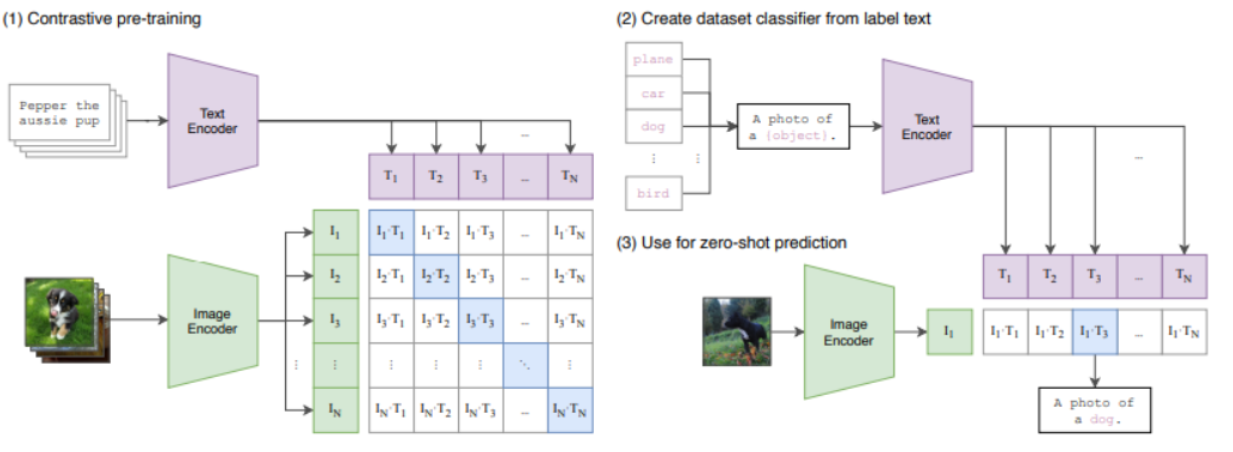
\includegraphics[width=\textwidth]{images/1-intro/clip.png}
    \caption{Embedding method proposed under the CLIP model \cite{radford2021learningtransferablevisualmodels}}
\end{figure}

However, the original CLIP model suffers from a limited context window size, which only allows for alignment with brief and concise captions.
This lacks the capability to align representations of images and their detailed long-form captions.
A later variant, Long-CLIP \cite{10.1007/978-3-031-72983-6_18}, resolves this issue by allowing the CLIP model to align to longer and more detailed natural language descriptions of images,
providing more robust alignment between text and images.

\paragraph{DINOv2 and Talk2DINO}
DINOv2 \cite{oquab2024dinov2learningrobustvisual} is a high-performing vision foundational model that can produce visual features from images.
The model is a Vision Transformer (ViT) model trained on a dataset of 142M images (LVD-142M), employing a self-supervised learning method.
Features generated from DINOv2 require no task-specific tuning to achieve state-of-the-art performance across various vision tasks,
such as segmentation, depth estimation, and matching across images.

While DINOv2 achieves high performance in fine-grained visual tasks, DINOv2 inherently lacks a connection to natural language.
Talk2DINO \cite{Barsellotti_2025_ICCV} leverages both the exceptional visual accuracy of DINOv2 and text embeddings of CLIP to fill this gap,
using a non-linear mapping layer to map CLIP embeddings to the DINOv2 embedding space.
This model enables state-of-the-art unsupervised open-vocabulary segmentation and produces superior segmentation masks.
The vision-language alignment performance of this model also makes it possible for text-to-image retrieval, using detailed prompts and captions.

\begin{figure}[H]
    \centering
    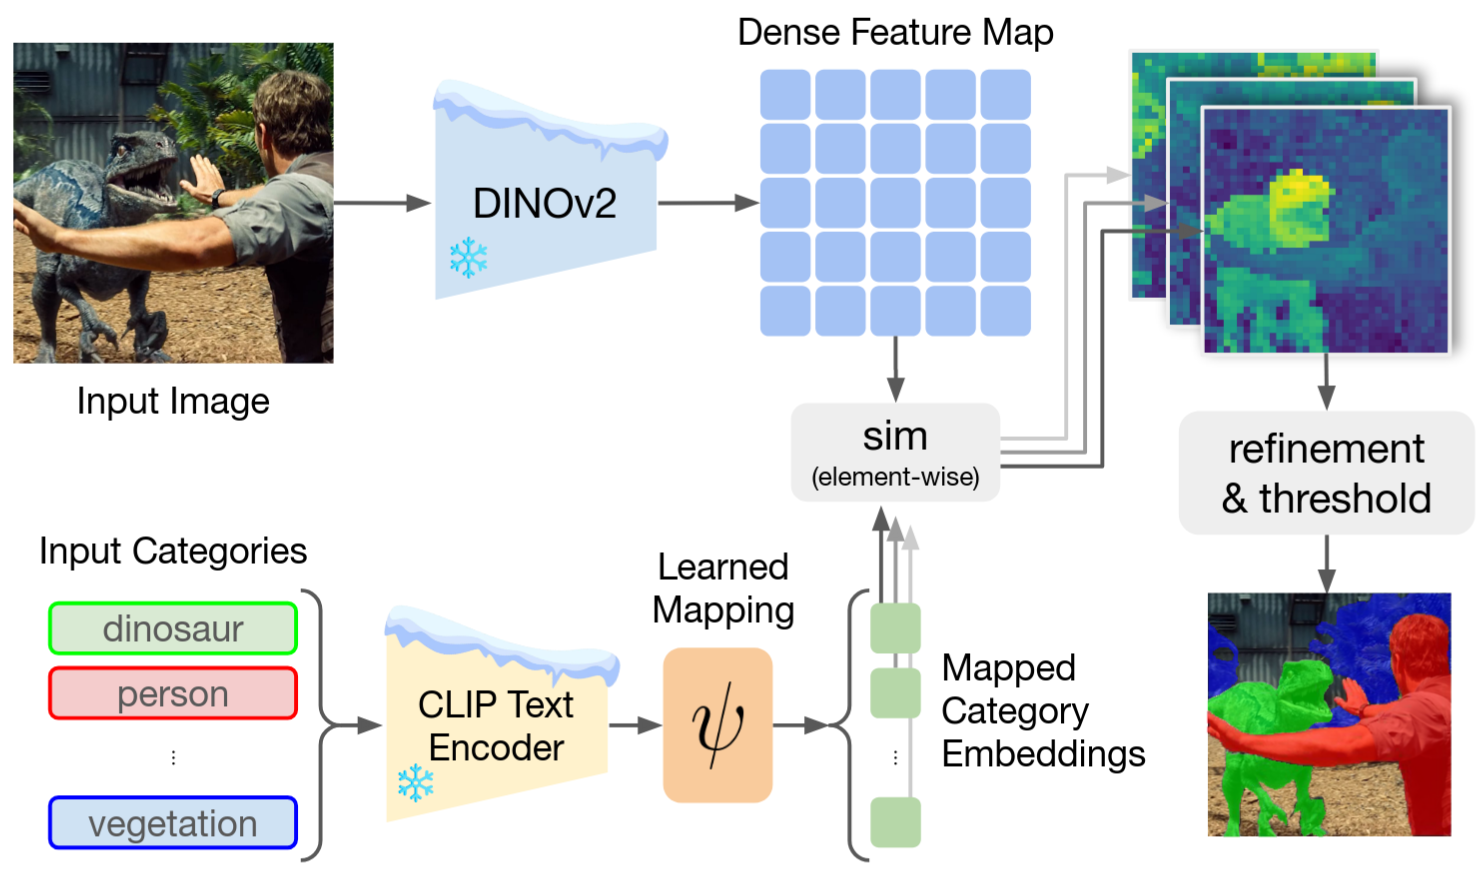
\includegraphics[width=0.7\textwidth]{images/1-intro/talk2dino-overview.png}
    \caption{Overview of Talk2DINO \cite{Barsellotti_2025_ICCV}}
\end{figure}

\paragraph{Positioning}
Unlike previous works that use CLIP to embed visual elements and lose fine-grained visual elements, 
or rely on text-based captions that discard visual information,
our pipeline uses Talk2DINO to query items in the DINOv2 embedding space using natural language, 
preserving fine-grained visual details while enabling text-based queries.

\subsubsection{Visual-RAG Benchmarks}

\paragraph{Visual-RAG}
Visual-RAG \cite{wu2025visualragbenchmarkingtexttoimageretrieval} focuses on text-to-image retrieval for knowledge-intensive queries,
using the iNaturalist 2021 \cite{Van_Horn_2021_CVPR} dataset (with 2.7M images of 10,000 different species).
Their findings revealed that noise in retrieved image batches may confuse MLLMs,
especially when the query targets visual evidence only present in a small region.
This motivates our preservation of raw visual features instead of flattening to image captions.

\begin{figure}
    \centering
    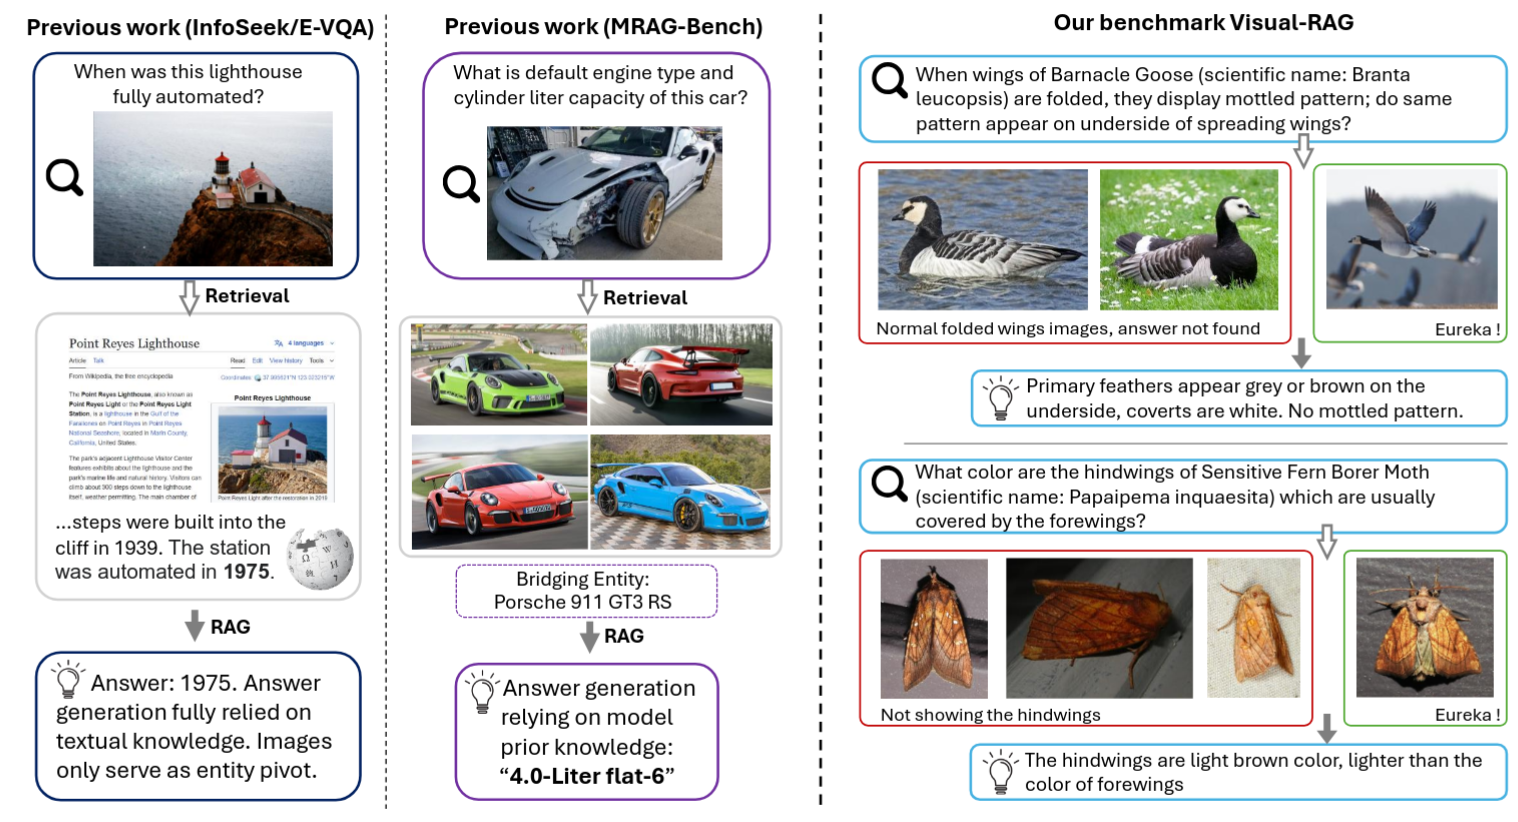
\includegraphics[width=\textwidth]{images/1-intro/visual-rag-bench.png}
    \caption{Comparison between previous benchmarks and Visual-RAG \cite{wu2025visualragbenchmarkingtexttoimageretrieval}}
\end{figure}

\paragraph{MMDocRAG}
MMDocRAG \cite{dong2025benchmarking} provides expert-annotated QA pairs requiring retrieval of multi-page or multi-document cross-modal evidence.
This benchmark tests end-to-end generation instead of retrieval-only evaluation.

\paragraph{Positioning}
Our work provides a complete end-to-end multimodal RAG pipeline that can be evaluated on retrieval and generation.
We use Visual-RAG and MMDocRAG to evaluate retrieval accuracy and end-to-end generation for our pipeline.

\subsubsection{Graph-based RAG}

\paragraph{GraphRAG} 
GraphRAG \cite{edge2025localglobalgraphrag} proposed using knowledge graphs for text-only RAG,
where entities form nodes, relationships between entites form edges, and community summaries generated by an LLM enable global sensemaking over document collections.

\paragraph{VideoRAG} 
VideoRAG \cite{ren2025videoragretrievalaugmentedgenerationextreme} extended the graph-based storage method to video content.
Captions of frames and video transcript are combined and transformed into a graph structure.
It was also shown that their methods in handling long-context content with graph representations demonstrate superior performance compared to existing methods.

\begin{figure}[H]
    \centering
    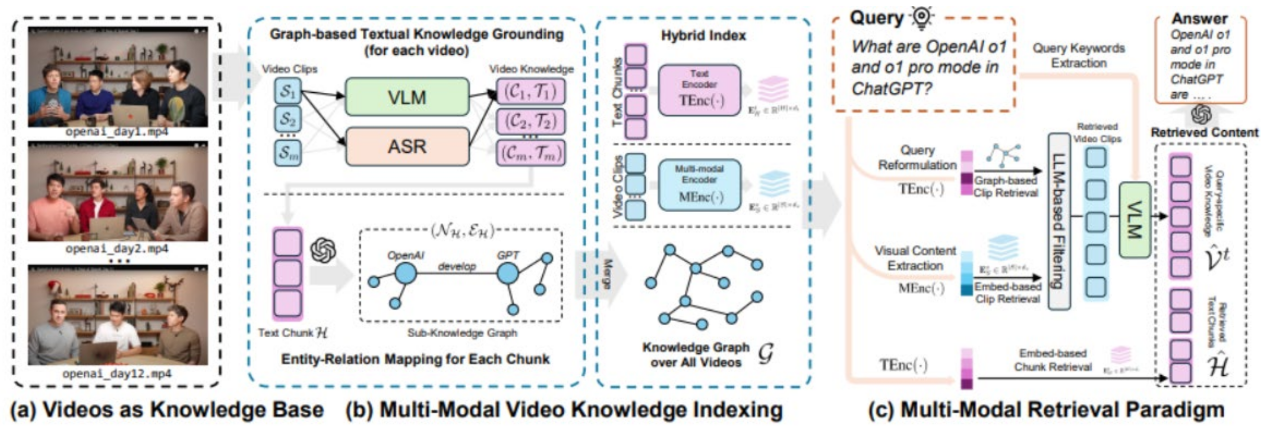
\includegraphics[width=\textwidth]{images/1-intro/video-rag.png}
    \caption{VideoRAG Framework for processing and retrieving video information \cite{ren2025videoragretrievalaugmentedgenerationextreme}}
\end{figure}

\paragraph{Positioning}
We adapt GraphRAG's community detection and summarization approach to our multimodal setting as an alternate configurable storage option.
Image entities are integrated as nodes linked via metadata to the visual vector database,
and retrieval can be performed either on dense vectors or graph communities, with configurable selection of storage methods.
This allows comparison between dense retrieval and graph-based retrieval on the same pipeline.

\subsubsection{Comparison with Prior Work}

\begin{tabular}{lcccc}
    \toprule
    \textbf{Feature} & \textbf{Text-only RAG} & \textbf{CLIP-based} & \textbf{VideoRAG \cite{ren2025videoragretrievalaugmentedgenerationextreme}} & \textbf{Ours} \\
    \midrule
    \textbf{Text retrieval} & \checkmark & \checkmark & \checkmark & \checkmark \\
    \textbf{Image retrieval} & \texttimes & \checkmark & \checkmark & \checkmark \\
    \textbf{Cross-modal} & \texttimes & \checkmark & \texttimes & \checkmark \\
    \textbf{Fine-grained visual features} & --- & \texttimes & \texttimes & \checkmark \\
    \textbf{Graph-based alternative} & \texttimes & \texttimes & \checkmark & \checkmark \\
    \bottomrule
\end{tabular}